\documentclass[a4paper,12pt]{report}
%
%			PREAMBOLO
%
\usepackage[a4paper]{geometry}
\usepackage{amssymb,amsmath,amsthm}
\usepackage{graphicx}
\usepackage{url}
\usepackage{hyperref}
\usepackage{epsfig}
\usepackage[italian]{babel}
\usepackage{setspace}
\usepackage{tesi}
\usepackage{float}
\usepackage{bussproofs}\EnableBpAbbreviations

% per inserire codice java
\usepackage{listings}

\lstset{
    language=Java,
    frame=single,
    breaklines=true,
    breakatwhitespace=true,
    tabsize=4,
    numbers=left,
    % numberstyle=\tiny
}

%per personalizzare i caption del listing
\usepackage{caption}
\DeclareCaptionLabelFormat{code}{Codice #2}
\captionsetup[lstlisting]{labelformat=code}

% per le accentate
\usepackage[utf8]{inputenc}
%
\newtheorem{myteor}{Teorema}[section]

\newenvironment{teor}{\begin{myteor}\sl}{\end{myteor}}

\usepackage{fancyhdr}
% Definizione del nuovo stile di pagina
\fancypagestyle{mystyle}{
    \fancyhf{} % Pulisce tutti i campi di intestazione e piè di pagina
    \fancyhead[R]{\thepage} % posiziona il numero di pagina in alto a destra della pagine
    \fancyhead[L]{\textsc{capitolo \thechapter}} % Posiziona il numero del capitolo a sinistra
    \renewcommand{\headrulewidth}{1pt} % Aggiunge la linea dell'intestazione
    \renewcommand{\footrulewidth}{0pt} % Rimuove la linea del piè di pagina
    \setlength{\headheight}{14.5pt}
}

\newcommand{\tto} {\leftrightarrow}

%
%
%			TITOLO
%
\begin{document}
\title{Implementazione in Java del metodo di risoluzione per la logica classica, ed estensione a logiche modali}
\author{Nicolò IACCARINO}
\dept{Corso di Laurea in Informatica} 
\anno{2023-2024}
\matricola{903870}
\relatore{Prof. Camillo FIORENTINI}
% 
%			DEDICA
%
\beforepreface
\prefacesection{Dediche}
        {\hfill \Large {\sl dedicato a \dots}}
% 
%			PREFAZIONE
%
\prefacesection{Prefazione}
...

%
%
%			ORGANIZZAZIONE
% \section*{Organizzazione della tesi}
% \label{organizzazione}
% La tesi \`e organizzata come segue:
% \begin{itemize}
% \item nel Capitolo \ref{intro} ....
% \end{itemize}

\afterpreface
\pagestyle{mystyle} %togli questo per ripristinare la numerazione del template
% 
% 
%			CAPITOLO 1
\chapter{Introduzione}
\label{intro}

\section{Panoramica generale}
Questo elaborato riguarda l'ambito della logica matematica, concentrandosi sul metodo di risoluzione per la logica classica, ovvero la logica proposizionale. Nel capitolo \ref{modal} verrà trattato il metodo di risoluzione per le logiche modali, che rappresentano un'estensione di quella proposizionale. Di seguito viene presentata una breve introduzione della logica proposizionale, utile a capire il funzionamento del metodo di risoluzione, trattato nel capitolo \ref{resol}.

\section{Logica proposizionale}

La logica proposizionale è un sistema formale per la rappresentazione e l'analisi del ragionamento, essa si basa su proposizioni. La sua sintassi comprende formule atomiche e formule composte. La semantica della logica proposizionale stabilisce come valutare le formule, associando loro valori di verità in base a interpretazioni che specificano lo stato di verità di ogni proposizione atomica.

\subsection{Formule atomiche}
Le formule atomiche rappresentano il caso più semplice di formula, nelle quali non vengono usati gli operatori logici. Una formula atomica è una variabile proposizionale, che può essere identificata tramite una lettera dell'alfabeto, ad esempio ``$p$''; essa viene valutata come vera (\emph{true}) o falsa (\emph{false}) in base all'interpretazione considerata. 

\subsection{Formule composte}
Le formule composte sono costruite mediante operatori logici (detti anche ``\emph{connettivi}'') a partire dalle formule atomiche. I connettivi della logica proposizionale sono:
\begin{itemize}
    \item $\lnot \;$ è la negazione logica (\textbf{not})
    \item $\land \;$ è la congiunzione logica (\textbf{and})
    \item $\lor \;$ è la disgiunzione logica (\textbf{or})
    \item $\to\;$ è l'implicazione logica (\textbf{implica})
    \item $\tto\;$ è la doppia implicazione (\textbf{se e solo se})
\end{itemize}
Consideriamo il seguente esempio di formula composta: 
\[ \lnot p \land q\] essa è ottenuta a partire dalla atomica ``$p$'' che viene negata tramite la negazione logica ($\lnot$), e successivamente messa in congiunzione logica ($\land$) con l'atomica ``$q$''. 
Si possono creare formule composte più complicate, in tal caso si usano le parentesi tonde per evitare ambiguità tra i connettivi.

L'interpretazione di una formula composta dipende dai connettivi usati e dall'interpretazione delle sue atomiche.

\subsection{Soddisfacibilità di una formula}
Una formula $F$ si dice \textbf{soddisfacibile} se e solo se ammette almeno un'interpretazione che la rende vera, ossia esiste almeno un assegnamento di valori di verità alle atomiche che rende vera $F$. Se tutte le interpretazioni possibili la rendono falsa, allora $F$ si dice \textbf{insoddisfacibile}.

\subsection{Tautologie e contraddizioni}
\label{taut-contr}
Una formula è una \textbf{tautologia} se e solo se ogni interpretazione della formula la rende vera. Quindi una tautologia è una formula sempre vera, che come vedremo, può essere ridondante in alcuni casi. Ad esempio, la formula ``$p \, \lor \, \lnot p$'' è il caso più semplice di tautologia.

Una formula è una \textbf{contraddizione} se e solo se è insoddisfacibile, ovvero tutte le sue interpretazioni la rendono falsa. Ad esempio, la formula ``$p \, \land \, \lnot p$'' è una contraddizione. \`E bene notare che se si applica la negazione logica ad una contraddizione si ottiene una tautologia, e viceversa.

% 
% 
%			CAPITOLO 2
\chapter{Il metodo di risoluzione per la logica classica}
\label{resol}
Il metodo di risoluzione è un sistema di calcolo logico per inferire la soddisfacibilità di una formula, esso ha avuto un impatto significativo in vari settori della matematica, dell'informatica e dell'ingegneria. È stato utilizzato per dimostrare teoremi importanti, risolvere problemi pratici e sviluppare algoritmi per l'intelligenza artificiale, la verifica formale e la progettazione dei circuiti. 

Questo metodo consiste nell'applicare più volte una sola regola: la regola di risoluzione. Il difetto è che essa opera soltanto su formule espresse in \textbf{Forma normale congiuntiva (CNF)}, ovvero come congiunzione di clausole. Prima di vedere il metodo di risoluzione è bene capire in che cosa consiste la \emph{CNF}.

\section{Forma normale congiuntiva}
\label{CNF}
\subsection{Letterali}
Un letterale è una formula atomica, oppure la sua negazione. Ad esempio ``$a$'' e ``$\lnot b$'' sono dei letterali, essi rappresentano l'elemento fondamentale delle clausole.

\subsubsection{Opposto di un letterale}
Dato un letterale $L$, il suo \emph{opposto} $\overline{L}$ è la sua negazione, ad esempio: se $L = p$ allora $\overline{L} = \lnot p$ e se $L = \lnot p$ allora $\overline{L} = p$.

\subsection{Clausole}
Una clausola è una disgiunzione di letterali. Consideriamo il seguente esempio:
\[ a \lor \lnot b \lor \lnot c \lor d \] 
questa è una clausola formata dai letterali ``$a$'', ``$\lnot b$'', ``$\lnot c$'', ``$d$''.

Una clausola può anche essere rappresentata in notazione insiemistica, in questo modo diventa un insieme di letterali. La clausola dell'esempio precedente diventa:
\[ \{a, \lnot b, \lnot c, d\}\]
che come si può notare, il simbolo di disgiunzione logica non è più presente, ma è sottinteso. D'ora in avanti useremo sempre la notazione insiemistica per rappresentare le clausole.

L'interpretazione delle clausole è semplice: una clausola è vera se e solo se almeno un letterale appartenente ad essa è vero in una data interpretazione (a causa della disgiunzione).

\subsubsection{Clausola tautologica}
Una clausola è una tautologia se e solo se contiene un letterale ed il suo opposto. Ad esempio: ``$\{ a, b, c, \lnot a \}$'' è una tautologia, perché contiene il letterale ``$a$'' ed il suo opposto. Infatti questo tipo di clausola risulta essere sempre vera, qualunque sia l'interpretazione dei suoi letterali (si veda la sezione \ref{taut-contr}).

\subsubsection{Clausola vuota}
è importante notare che una clausola può non contenere alcun letterale, in tal caso si parla di \emph{clausola vuota}. La clausola vuota rappresenta la \textbf{contraddizione} (si veda la sezione \ref{taut-contr}) e si può indicare con ``$\{ \}$''.

\subsection{Insiemi di clausole}
La \emph{CNF} consiste in una congiunzione di clausole. Seguendo lo stesso approccio per le clausole, la \emph{CNF} può essere rappresentata anch'essa in notazione insiemistica come \textbf{insieme di clausole}, quindi ad esempio la seguente \emph{CNF}:
\[ (a \lor b) \land (\lnot a \lor c) \land (\lnot b \lor c) \]
diventa
\[\{ \; \{a, b\}, \{\lnot a, c\}, \{\lnot b, c\} \; \}\]
anche in questo caso la congiunzione è sottintesa. Possiamo quindi considerare la \emph{CNF} e gli insiemi di clausole come lo stesso oggetto semantico.

\subsubsection{Soddisfacibilità di un insieme di clausole}
Un insieme di clausole $S$ è \textbf{soddisfacibile} se e solo se esiste almeno un'interpretazione che rende vere \textbf{tutte} le clausole appartenenti a $S$ (a causa della congiunzione).

\section{Regola di risoluzione}
La regola di risoluzione, che chiamiamo Res, è una regola di inferenza che, a partire da due clausole di premessa, genera una clausola conclusione (detta \textbf{risolvente}). Per poter applicare \emph{Res} su due clausole $C_1$ e $C_2$, è necessario che esista un letterale $L \in C_1$ ed il suo opposto $\overline{L} \in C_2$. Se questo non dovesse capitare, allora la regola non è applicabile su $C_1$ e $C_2$.

\subsection{Clausola risolvente}
Per poter ottenere la clausola risolvente (\emph{R}) si rimuove il letterale $L$ dalla clausola $C_1$ ed il suo opposto $\overline{L}$ dalla clausola $C_2$, infine si uniscono le due clausole (con l'operazione di \textbf{unione} insiemistica). Vediamo un esempio:

\[
    \AXC{$\overbrace{\{ a, b \}}^{C_1}$}
    \AXC{$\overbrace{\{\lnot b, c, d \}}^{C_2}$}
    \RightLabel{Res}
    \BIC{$\underbrace{\{ a, c, d \}}_{R}$}
    \DP
\]
la risolvente \emph{R} è stata ottenuta cancellando il letterale ``$b$'' (da $C_1$) ed il suo opposto ``$\lnot b$'' (da $C_2$), e facendo l'unione.

\section{Funzionamento del metodo di risoluzione}
Il metodo di risoluzione opera su un insieme $S$ di clausole, e applica (dove possibile) \emph{Res} su tutte le coppie di clausole appartenenti a $S$ con lo scopo di trovare la contraddizione (clausola vuota). Ogni volta che il metodo applica \emph{Res}, la risolvente viene aggiunta a $S$, la quale potrà poi essere considerata come clausola di premessa per una successiva applicazione di \emph{Res}. Se il metodo riesce a trovare la clausola vuota, allora prova che $S$ è \textbf{insoddisfacibile}; se invece, dopo aver applicato \emph{Res} su tutte le possibili coppie di clausole non la trova, allora il metodo prova che $S$ è \textbf{soddisfacibile}.

\subsection{Gestione delle clausole tautologiche}
Nella \emph{CNF} le clausole tautologiche rappresentano una ridondanza, perché essendo la \emph{CNF} una congiunzione di clausole, esse non indicano alcun valore informativo. Questo si traduce col fatto che nel metodo di risoluzione si possono ignorare questo tipo di clausole, rendendo più semplice l'esecuzione del metodo anche da un punto di vista computazionale (come vedremo nel capitolo \ref{impl}).

Un altro aspetto da tenere in considerazione è che applicando \emph{Res} è possibile che la risolvente sia una tautologia, in tal caso la risolvente viene scartata (non viene aggiunta a $S$). Vediamo un esempio di clausole $C_1$ e $C_2$ che generano una risolvente $R$ tautologica:

\[
    \AXC{$\overbrace{\{ a, \lnot b \}}^{C_1}$}
    \AXC{$\overbrace{\{\lnot a, b \}}^{C_2}$}
    \RightLabel{Res}
    \BIC{$\underbrace{\{ \lnot b, b \}}_{R}$}
    \DP
\]
per ottenere $R$ è stato rimosso il letterale $a$ ed il suo opposto. Si può notare che in questo caso si poteva anche considerare il letterale $\lnot b \in C_1$ ed il suo opposto $b \in C_2$ ed ottenere $R^{'} = \{ \lnot a, a \}$, ma dal punto di vista del metodo di risoluzione non cambia nulla perché $R$ e $R^{'}$ sono entrambe tautologie, e quindi scartate.

\subsection{Esempio pratico del metodo di risoluzione}
\subsubsection{Esempio su un insieme di clausole insoddisfacibile}
Consideriamo il seguente insieme di clausole $S$:
\[ S = \{ \; \{a\}, \{\lnot a, b\}, \{\lnot b\} \; \} \]
in questo caso la contraddizione si ricava applicando due volte \emph{Res}:

\begin{itemize}
    \item \textbf{Step 1:}
    \[
    \AXC{$\overbrace{\{ a \}}^{C_1}$}
    \AXC{$\overbrace{\{\lnot a, b \}}^{C_2}$}
    \RightLabel{Res}
    \BIC{$\underbrace{\{ b \}}_{R}$}
    \DP
    \]
    \item \textbf{Step 2:}
    \[
    \AXC{$\overbrace{\{ b \}}^{C_1}$}
    \AXC{$\overbrace{\{\lnot b \}}^{C_2}$}
    \RightLabel{Res}
    \BIC{$\underbrace{\{\}}_{R}$}
    \DP
    \]
\end{itemize}
nello \emph{Step 2} la regola \emph{Res} ha trovato la clausola vuota, questo dimostra che $S$ è \textbf{insoddisfacibile}. Si noti che la clausola $C_1$ dello \emph{Step 2} è la risolvente $R$ dello \emph{Step 1}.

\subsubsection{Esempio su un insieme di clausole soddisfacibile}
Consideriamo ora il seguente insieme di clausole $S^{'}$:
\[ S^{'} = \{ \; \{a\}, \{\lnot a, b\}, \{\lnot c\} \; \} \]
in questo caso il metodo di risoluzione applica una sola volta \emph{Res}:
\[
    \AXC{$\overbrace{\{ a \}}^{C_1}$}
    \AXC{$\overbrace{\{\lnot a, b \}}^{C_2}$}
    \RightLabel{Res}
    \BIC{$\underbrace{\{ b \}}_{R}$}
    \DP
\]
% \[ C_1 = \{a\} \] \[ C_2 = \{\lnot a, b\} \] \[ \rule{4cm}{0.2pt} \] \[R = \{b \}\]
stavolta, il metodo non riesce più ad andare avanti, perché \emph{Res} non è più applicabile in nessun'altra coppia di clausole presenti in $S^{'}$, anche tenendo conto della clausola $R$ appena generata. Questo significa che la contraddizione non può essere ricavata, e quindi $S^{'}$ è \textbf{soddisfacibile}.

% 
% 
%			CAPITOLO 3
\chapter{Implementazione in Java del metodo di risoluzione}
\label{impl}

Questo capitolo si concentra sull'implementazione pratica del metodo di risoluzione per la logica classica in linguaggio Java. Esploreremo come tradurre i concetti teorici esaminati nei capitoli precedenti in codice eseguibile, analizzando le classi, i metodi e le strutture dati necessari per realizzare efficacemente il metodo di risoluzione. Partiremo con una panoramica generale dell'architettura del progetto Java, identificando le principali classi per rappresentare le strutture dati necessarie per il metodo di risoluzione. Successivamente, affronteremo la classe che implementa l'algoritmo di risoluzione. Nel capitolo \ref{formulas} vedremo l'implementazione delle formule della logica proposizionale e la loro conversione in \emph{CNF}.

\section{Struttura del progetto Java}
\label{project_structure}

Di seguito viene mostrato l'elenco dei package contenuti nella directory \emph{src} del progetto, e i file java contenuti in ognuno di essi:
\begin{itemize}
    \item \textbf{literal}
        \begin{itemize}
            \item \emph{Literal.java}
            \item \emph{Atom.java}
            \item \emph{NegAtom.java}
        \end{itemize}
    \item \textbf{cnf}
        \begin{itemize}
            \item \emph{Clause.java}
            \item \emph{ClauseSet.java}
        \end{itemize}
    \item \textbf{resolution}
        \begin{itemize}
            \item \emph{Resolution.java}
            \item \emph{Step.java}
        \end{itemize}
    \item \textbf{formula}
        \begin{itemize}
            \item \emph{Formula.java}
            \item \emph{AtomicFormula.java}
            \item \emph{CompoundFormula.java}
        \end{itemize}
    \item \textbf{connective}
        \begin{itemize}
            \item \emph{Connective.java}
        \end{itemize}
    \item \textbf{antlr4}
        \begin{itemize}
            \item \emph{FormulaExpression.g4}
            \item \emph{FormulaExpressionListener.java}
            \item \emph{FormulaExpressionBaseListener.java}
            \item \emph{FormulaExpressionLexer.java}
            \item \emph{FormulaExpressionParser.java}
            \item \emph{FormulaListenerImplementation.java}
            \item \emph{ParseFormula.java}
        \end{itemize}
    \item \textbf{test}
        \begin{itemize}
            \item \emph{ResolutionTest.java}
            \item (file \emph{txt} per il test)
        \end{itemize}
    \item \emph{App.java}
\end{itemize}
In questo capitolo ci concentriamo sui primi tre package dell'elenco, che sono i principali per l'implementazione del metodo di risoluzione. Gli altri package contengono le classi per rappresentare le formule, eseguire il parsing delle formule, effettuare il testing, ed infine è presente file \emph{App.java} che contiene il metodo \emph{main} (si noti che questa classe non è contenuta in alcun package).


\section{Strutture dati per la CNF}
I package ``\textbf{literal}'' e ``\textbf{cnf}'' contengono le classi per rappresentare la CNF, fondamentali per il metodo di risoluzione.

\subsection{La classe astratta Literal e le classi Atom e NegAtom}
La classe \texttt{Literal} permette di rappresentare i letterali. Essa è una classe astratta che fornisce un'interfaccia comune per le classi \texttt{Atom} e \texttt{NegAtom}, che la estendono per rappresentare rispettivamente una variabile atomica e la negazione di essa. Questo approccio consente una gestione modulare dei letterali, facilitando l'estensione e il mantenimento del codice. La classe \texttt{Literal} contiene una stringa come campo privato che identifica il nome del letterale, e il corrispettivo metodo \texttt{getName()} che lo restituisce; inoltre, ha un metodo astratto \texttt{getOpposite()} sovrascritto dalle due classi che la estendono, che permette di restituire l'opposto del letterale sul quale viene chiamato (se chiamato su un'istanza di \texttt{Atom} restituisce l'istanza corrispondente di \texttt{NegAtom}, e viceversa). Il metodo \texttt{toString} della classe \texttt{NegAtom} usa il carattere ``\textbf{$\sim $}'' per rappresentare testualmente la negazione logica in un atomo negato (ad esempio ``\emph{$\sim p$}'').

\begin{minipage}{\linewidth}
    \begin{lstlisting}[title={metodo getOpposite sovrascritto dalla classe Atom}]
        @Override
        public Literal getOpposite() {
            return new NegAtom(this.getName());
        }
    \end{lstlisting}
\end{minipage}

\subsection{La classe Clause}
Questa classe permette di rappresentare le clausole della \emph{CNF}, tenendo conto della loro notazione insiemistica. La classe contiene il campo \texttt{literals} di tipo \texttt{Set<Literal>} che consiste nell'insieme di letterali, inoltre contiene anche il campo \texttt{index} che rappresenta un indice numerico che identifica la clausola istanziata.

All'interno della classe \emph{Clause} sono presenti i classici metodi per gli insiemi (\texttt{add}, \texttt{remove}, \texttt{contains}, ecc.), in aggiunta al metodo \texttt{union} che permette di eseguire l'unione insiemistica con un'altra clausola specificata come parametro. Un altro importante metodo è \texttt{isTautology} che restituisce \emph{true} se e solo se la clausola è una tautologia (si veda il codice \ref{istaut}). La classe \emph{Clause} segue il design pattern ``iterator'', che permette di iterare facilmente sui letterali di una clausola tramite il ciclo \emph{for-each} di Java.

\begin{minipage}{\linewidth}
    % \small
    \begin{lstlisting}[caption={Metodo isTautology della classe Clause}, label={istaut}]
        public boolean isTautology() {
            for (Literal l1 : this.literals) {
                for (Literal l2 : this.literals) { 
                    if (l1.equals(l2.getOpposite())) return true;
                }
            }
            return false;
        }
    \end{lstlisting}
\end{minipage}
Questo codice mostrato esegue un doppio loop sulla clausola (utilizzando il campo \texttt{literals}) per verificare la presenza di un letterale ed il suo opposto all'interno di essa. Se questo dovesse capitare, allora la clausola è una tautologia e il metodo restituisce \emph{true}; altrimenti restituisce \emph{false} dopo aver terminato il doppio loop.

\subsection{La classe ClauseSet}
Questa classe rappresenta la \emph{CNF} in notazione insiemistica, ovvero gli insiemi di clausole. Nella classe è presente il campo \texttt{clauses} di tipo \texttt{Set<Clause>}, che contiene le clausole dell'istanza di \emph{ClauseSet}. Anche in questo caso ci sono i metodi per gestire gli elementi dell'insieme come nella classe \emph{Clause}, ed il metodo \texttt{union} per fare l'unione insiemistica dell'oggetto con un'altra istanza di \emph{ClauseSet}. Importante è il metodo \texttt{removeTautologies} che rimuove le clausole tautologiche dall'oggetto, in questo modo si tolgono le ridondanze, rendendo più semplice la \emph{CNF} (si veda il codice \ref{remtaut}). Anche la classe \emph{ClauseSet} segue il design pattern ``iterator''.

\begin{minipage}{\linewidth}
    \small
    \begin{lstlisting}[caption={Metodo ``removeTautologies'' della classe ClauseSet}, label={remtaut}]
        public void removeTautologies() {
            List<Clause> tautologies = new ArrayList<>();
            for (Clause c : this.clauses) {
                if (c.isTautology()) {
                    tautologies.add(c);
                }
            }
            for (Clause taut : tautologies) {
                this.clauses.remove(taut);
            }
        }
    \end{lstlisting}
\end{minipage}
Questo codice esegue la rimozione delle clausole tautologiche: prepara una lista \texttt{tautologies} vuota, esegue un loop sul campo \texttt{clauses} per aggiungere alla lista le tautologie, ed infine esegue un loop sulla lista \texttt{tautologies} per rimuovere le tautologie contenute in \texttt{clauses}.

\section{La classe Resolution}
La classe \emph{Resolution} è una classe senza costruttori che contiene alcuni campi statici e metodi statici per l'implementazione del metodo di risoluzione. I campi della classe sono tre:
\begin{itemize}
    \item \texttt{visited}: è di tipo \texttt{Map<Integer, Set<Integer>>} e consiste in una mappa che associa una clausola ad un insieme di clausole (utilizzando i loro indici). Essa memorizza tutte le clausole alle quali è stata applicata la regola di risoluzione con la clausola rappresentata dalla chiave della mappa (si veda la sottosezione \ref{visited}).
    \item \texttt{enableSteps}: è un campo booleano che, se impostato a \texttt{true}, permette di abilitare i passaggi del metodo di risoluzione quando viene eseguito (si veda la sottosezione \ref{step}).
    \item \texttt{trace}: è una lista di \texttt{Step}, che memorizza tutti i passaggi del metodo di risoluzione se il campo \texttt{enableSteps} è impostato a \texttt{true} (si veda la sottosezione \ref{step}).
\end{itemize}

I metodi statici della classe sono:
\begin{itemize}
    \item \texttt{isSatisfiable} (spiegato nella sottosezione \ref{isSat})
    \item \texttt{getComplementaryLiteral} (spiegato nella sottosezione \ref{isSat})
    \item \texttt{alreadyVisited} (spiegato nella sottosezione \ref{visited})
    \item \texttt{resolRule} (spiegato nella sottosezione \ref{resolRule})
    \item \texttt{setEnableSteps} (spiegato nella sottosezione \ref{step})
    \item \texttt{printTrace} (spiegato nella sottosezione \ref{step})
\end{itemize}

\subsection{Il metodo ``isSatisfiable''}
\label{isSat}
Questo è il metodo più importante della classe \emph{Resolution}. Esso ha come parametro in input un oggetto ClauseSet \texttt{s} e restituisce \texttt{true} se \texttt{s} è soddisfacibile, \texttt{false} altrimenti. Di seguito viene mostrato il codice. Il metodo \emph{isSatisfiable} dopo aver controllato che \texttt{s} non sia \texttt{null} o un insieme vuoto, elimina tutte le clausole tautologiche appartenenti a \texttt{s} richiamando il metodo \texttt{removeTautologies} sull'oggetto \texttt{s}. Successivamente controlla che sia vuoto (in tal caso viene restituito \texttt{true} perché \texttt{s} è una tautologia), e in caso negativo continua l'esecuzione inizializzando i campi \texttt{visited} e \texttt{trace}; inoltre, le clausole in \texttt{s} vengono inserite nella lista di clausole \texttt{listCl} per poter consentire la modifica della lista durante il suo scorrimento (eseguito dal ciclo \emph{for}). 

A questo punto vengono eseguiti due cicli for innestati su \texttt{listCl}; il ciclo esterno itera la lista utilizzando la clausola \texttt{c1}, il ciclo interno utilizza la clausola \texttt{c2}. Il codice \ref{double-for} mostra l'esecuzione dei due cicli. 

% \begin{figure}[]
    
\begin{minipage}{\linewidth}
\small 
\begin{lstlisting}[caption={Metodo ``isSatisfiable'' della classe Resolution}, label={double-for}]
        for (int i = 0; i < listCl.size(); i++) {
            Clause c1 = listCl.get(i);
            int index1 = c1.getIndex();
            for (int j = 0; j < listCl.size(); j++) {
                Clause c2 = listCl.get(j);
                int index2 = c2.getIndex();
                if ((i != j) && !alreadyVisited(c1, c2)) {
                    Literal complemLit = getComplementaryLiteral(c1, c2);
                    if (complemLit != null) {
                        if (index1 < index2) {
                            (visited.get(index1)).add(index2);
                        } else {
                            (visited.get(index2)).add(index1);
                        }
                        Clause resolvent = resolRule(c1, c2, complemLit);
                        Step step = null;
                        if (enableSteps) {
                            step = new Step(c1, c2, resolvent, complemLit);
                            trace.add(step);
                        }
                        if (resolvent.isEmpty()) {
                            if (enableSteps) printTrace();
                            return false;
                        } 
                        if (resolvent.isTautology()) {
                            if (enableSteps)
                                step.setTautology();
                        } else if (listCl.contains(resolvent)) {
                            if (enableSteps)
                                step.setAlreadyPresent();
                        } else {
                            visited.put(resolvent.getIndex(), new HashSet<>());
                            listCl.add(resolvent);
                        }
                    }
                }
            }
        }
        if (enableSteps) printTrace();
        return true;
    }
\end{lstlisting}
\end{minipage}
% \end{figure}

Una volta entrato nel secondo ciclo, il metodo esegue la regola di risoluzione (metodo \texttt{resolRule}) su \texttt{c1} e \texttt{c2}, se e solo se le due clausole non sono uguali, non sono già state visitate in precedenza, e contengono almeno un letterale complementare in comune (metodo \texttt{getComplementaryLiteral}). Una volta eseguita la regola sulle due clausole, viene controllato se la clausola \texttt{resolvent} è vuota (metodo \texttt{isEmpty}); in tal caso il metodo restituisce \texttt{false} e termina la sua esecuzione, altrimenti la continua e aggiunge la risolvente a \texttt{listCl} se e solo se \texttt{resolvent} non è tautologica e non è già presente nella lista. A questo punto si esegue la successiva iterazione del \texttt{for} interno.

\subsubsection{Il metodo ``getComplementaryLiteral''}
Questo metodo controlla se nella clausola \texttt{c1} è presente un letterale \texttt{l1}, ed il suo opposto \texttt{l2} nella clausola \texttt{c2}. Se lo trova lo restituisce, altrimenti restituisce \texttt{null}. Il codice \ref*{gcl} mostra questo metodo. 

\begin{minipage}{\linewidth}
    \begin{lstlisting}[caption={Metodo ``getComplementaryLiteral'' della classe Resolution}, label={gcl}]
        private static Literal getComplementaryLiteral(Clause c1, Clause c2) { 
            for (Literal l1 : c1) {
                for (Literal l2 : c2) { 
                    if (l1.equals(l2.getOpposite())) return l1;
                }
            }
            return null;
        }
    \end{lstlisting}
\end{minipage}

\subsection{Memorizzazione delle coppie di clausole visitate}
\label{visited}
Per evitare che si esegua la regola di risoluzione più di una volta su una stessa coppia di clausole, è opportuno memorizzare la coppia sulla mappa \texttt{visited}. Essa utilizza gli indici delle clausole, ed ha come chiave un \texttt{Integer}, e come valore un insieme di interi (\texttt{Set<Integer>}). Ogni volta che viene eseguita la regola di risoluzione su \texttt{c1} e \texttt{c2}, viene aggiunto l'indice più grande alla mappa ottenuta come valore a partire dalla chiave corrispondente all'indice più piccolo. In questo modo viene gestita più semplicemente la simmetria, infatti se \texttt{c1} e \texttt{c2} sono già state visitate, allora vale la stessa cosa anche per \texttt{c2} e \texttt{c1}. Nel codice \ref{double-for} L'inserimento degli indici nella mappa viene eseguito tra la riga 10 e la riga 14.

\subsubsection{Esempio di funzionamento della mappa}
Consideriamo il seguente insieme di clausole con associati gli indici ad ognuna di essa:

% \vspace{10pt}

\begin{center}
\begin{tabular}{|c||c|c|c|}
    \hline
    \textbf{Clausole} & $\{a, \lnot b, c\}$ & $\{\lnot a, d\}$ & $\{\lnot c\}$ \\
    \hline
    \textbf{Indici} & 0 & 1 & 2 \\
    \hline
\end{tabular}
\end{center}
\vspace{10pt}
In questo caso, il metodo \texttt{isSatisfiable} richiama il metodo \texttt{resolRule} sulle clausole \textbf{0} e \textbf{1}, e crea la risolvente con indice \textbf{3}. Nella mappa viene aggiunto \textbf{1} nell'insieme corrispondente alla chiave \textbf{0} (perché $0 < 1$). Poi va avanti eseguendo altre volte la regola; le clausole che vengono aggiunte all'insieme di partenza sono le seguenti:

% \vspace{10pt}

\begin{center}
    \begin{tabular}{|c||c|c|c|}
        \hline
        \textbf{Clausole} & $\{\lnot b, c, d\}$ & $\{a, \lnot b\}$ & $\{d, \lnot b\}$ \\
        \hline
        \textbf{Indici} & 3 & 4 & 5 \\
        \hline
    \end{tabular}
\end{center}
\vspace{10pt}
Nella situazione finale la mappa visited avrà la seguente struttura:

\vspace{10pt}

\begin{center}
    \begin{tabular}{|c|c|}
        \hline
        \multicolumn{1}{|c|}{\textbf{Chiavi}} & \multicolumn{1}{c|}{\textbf{Valori}} \\
        \hline\hline
        0 & $\{1, 2\}$ \\
        1 & $\{4\}$ \\
        2 & $\{3\}$ \\
        \hline
    \end{tabular}
\end{center}
\vspace{10pt}
La prima riga dice che la clausola \textbf{0} è stata visitata con le clausole \textbf{1} e \textbf{2} (infatti le clausole \textbf{3} e \textbf{4} sono state ottenute dalle coppie \textbf{0 - 1} e \textbf{0 - 2}). La seconda riga dice che la clausola \textbf{1} è stata visitata con la clausola \textbf{4} (per ottenere la clausola \textbf{5}); infine, la terza riga dice che la clausola \textbf{2} è stata visitata con la clausola \textbf{3} (in quest'ultimo caso viene generata la clausola \textbf{6} che è uguale alla clausola \textbf{5}, quindi viene scartata).

\subsubsection{Il metodo ``alreadyVisited''}
Questo metodo utilizza la mappa \texttt{visited} per verificare se una coppia di clausole è gia stata visitata in precedenza, ossia la regola di risoluzione è già stata applicata su di essa. Per farlo controlla se nell'insieme ottenuto dall'indice più piccolo è presente l'indice più grande (utilizzando il metodo \texttt{contains}). Questo garantisce che l'algoritmo possa terminare. Il codice \ref{alreadyVisited} mostra questo metodo.

\begin{minipage}{\linewidth}
    % \small
    \begin{lstlisting}[caption={Metodo ``alreadyVisited'' della classe Resolution}, label={alreadyVisited}]
        private static boolean alreadyVisited(Clause c1, Clause c2) {
            int i1 = c1.getIndex();
            int i2 = c2.getIndex();
            if (i1 < i2) {
                return (visited.get(i1)).contains(i2);
            }
            return (visited.get(i2)).contains(i1);
        }
    \end{lstlisting}
\end{minipage}

\subsection{Implementazione della regola di risoluzione}
\label{resolRule}
La regola \emph{Res} viene implementata dal metodo \texttt{resolRule}; esso prende in input le clausole \texttt{c1} e \texttt{c2}, insieme al letterale \texttt{lit}. Il metodo esegue l'unione delle due clausole (tramite il metodo \texttt{union} della classe \texttt{Clause}), e successivamente rimuove il letterale \texttt{lit} ed il suo opposto dalla clausola risultante; infine restituisce il risultato. Il codice \ref{rr} mostra questo metodo.

\begin{minipage}{\linewidth}
    \begin{lstlisting}[caption={Metodo ``resolRule'' della classe Resolution}, label={rr}]
        private static Clause resolRule(Clause c1, Clause c2, Literal lit) {
            Clause result = c1.union(c2);
            result.remove(lit);
            result.remove(lit.getOpposite());
            return result;
        }
    \end{lstlisting}
\end{minipage}

\subsection{Gestione degli step}
\label{step}
Per verificare la correttezza dell'implementazione del metodo di risoluzione è possibile tenere traccia di tutti gli step che vengono eseguiti dal metodo \texttt{isSatisfiable}, ovvero di tutte le applicazioni della regola di risoluzione. Per farlo è stata scritta la classe \texttt{Step}, le cui istanze memorizzano il numero di step attuale, le due clausole di premessa, la clausola risolvente, il letterale da considerare per la regola, ed infine le informazioni che dicono che la risolvente viene scartata perché è tautologica oppure già presente nella lista di clausole.

Nella classe \texttt{Resolution} è presente il metodo \texttt{setEnableSteps} che prende in input un valore booleano che viene impostato sul campo statico \texttt{enableSteps}. Se questo campo è impostato a \texttt{true}, verrà stampata su Standard Output (\emph{Stdout}) la lista degli step quando viene chiamato il metodo \texttt{isSatisfiable}.

Gli step vengono memorizzati nel campo statico \texttt{trace} (di tipo \texttt{List<Step>}). Nel codice \ref{double-for}, nelle righe 16-19 viene creata una nuova istanza di \texttt{Step} e aggiunta a \texttt{trace} soltanto nel caso in cui il campo \texttt{enableSteps} è \texttt{true}. Nelle righe 25-30 viene controllato se la clausola risolvente è tautologica oppure è già presente in \texttt{listCl}, e vengono chiamati i metodi \texttt{setTautology} o \texttt{setAlreadyPresent} sullo step, per indicare che in quello step la risolvente viene scartata, specificandone il suo motivo. Nella riga 22 e nella riga 39 viene richiamato il metodo \texttt{printTrace}; esso itera sulla lista \texttt{trace}, stampando tutti gli step su \emph{Stdout}. 

\subsubsection{Esempio di funzionamento degli step}
Supponendo che il campo \texttt{enableSteps} sia impostato a \texttt{true}, consideriamo l'esecuzione del metodo \texttt{isSatisfiable} con il seguente insieme di clausole \texttt{s} in input:
\[\texttt{s} = \{\; \{a\}; \{\lnot a, b\}; \{\lnot b\} \;\}\]
La lista degli step che verrà stampata su \emph{Stdout} è la seguente:
\begin{figure}[H]
    \centering
    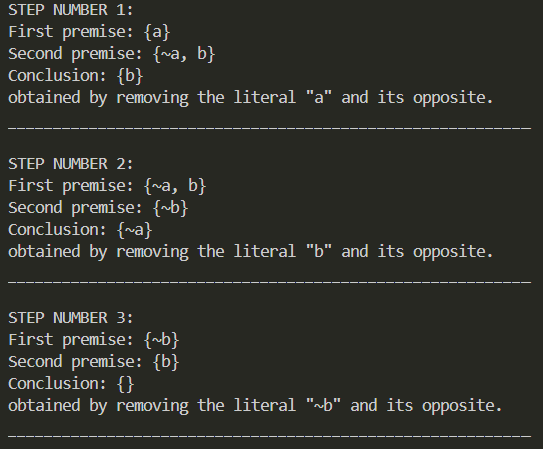
\includegraphics[width=0.7\textwidth, height=0.4\textheight]{img/step.png}
\end{figure} 
Come si può notare, nello \emph{step 3} viene trovata la clausola vuota, quindi in questo caso il metodo restituisce \texttt{false} (\texttt{s} è \emph{insoddisfacibile}).


% 
% 
%			CAPITOLO 4
\chapter{Implementazione in Java di formule generiche}
\label{formulas}
Finora ci siamo concentrati soltanto su formule espresse in \emph{CNF} rappresentate mediante la classe \texttt{ClauseSet}. Se volessimo implementare una formula qualsiasi della logica proposizionale sono necessari altri elementi. I package \emph{formula} e \emph{connective} del progetto java visto nella sezione \ref{project_structure} contengono i file necessari per rappresentare le formule della logica proposizionale. Se si volesse verificare la soddisfacibilità di una formula, è necessario convertire prima la formula in \emph{CNF} (ottenendo così l'istanza di \texttt{ClauseSet} associata), e poi richiamare il metodo \texttt{isSatisfiable} della classe \texttt{Resolution} dando in input quella istanza. Questo aspetto viene affrontato nella sezione \ref{clausification}.

\section{La classe astratta Formula}
Come visto nel capitolo \ref{intro}, una formula può essere \emph{atomica} o \emph{composta}, perciò nell'implementazione in Java è stata scritta la classe astratta \texttt{Formula}, che viene estesa dalle classi concrete \texttt{AtomicFormula} e \texttt{CompoundFormula}.

La classe \texttt{Formula} contiene soltanto il metodo astratto \texttt{toCnf} che permette di convertire la formula in \emph{CNF}, restituendo l'istanza di \texttt{ClauseSet} corrispondente (si veda la sezione \ref{clausification}).

\section{La classe AtomicFormula}
Questa classe estende \texttt{Formula} ed istanzia una formula atomica. Essa contiene un campo \texttt{atm} di tipo \texttt{Atom} che lo identifica, e alcuni semplici metodi per la sua gestione: il metodo per ottenere il nome (\texttt{getName}), il metodo per ottenere il letterale associato (\texttt{toLiteral}), e i classici metodi \texttt{equals} e \texttt{toString}.

\section{L'enumerazione Connective}
Prima di considerare la classe \texttt{CompoundFormula} è bene vedere prima l'enumerazione \texttt{Connective}. Essa si trova nel package \emph{connective} e definisce delle costanti enumerative che descrivono i connettivi della logica proposizionale usati dalle formule composte. La seguente tabella mostra le costanti associate alla loro rappresentazione testuale (ottenute dal metodo \texttt{toString}):
\begin{table}[H]
    \centering
    \begin{tabular}{|c||c|}
        \hline
        \textbf{Costante enumerativa} & \textbf{Rappresentazione testuale} \\
        \hline\hline
        NOT & $\sim$ \\
        \hline
        AND & $\&$ \\
        \hline
        OR & $|$ \\
        \hline
        IMPLIES & $->$ \\
        \hline
        IFF & $<->$ \\
        \hline
    \end{tabular}
\end{table}

\section{La classe CompoundFormula}
Questa classe estende \texttt{Formula} ed istanzia una formula composta, utilizzando le costanti dell'enumerazione \texttt{Connective}. Per la rappresentazione interna di una formula composta si usa un albero binario, che definisce la sua struttura ricorsiva. La radice dell'albero contiene il connettivo principale della formula, i nodi interni contengono i connettivi delle sue sottoformule, ed infine le foglie contengono le sue formule atomiche. I nodi che contengono i connettivi binari hanno due figli, mentre i nodi che contengono i connettivi unari hanno un solo figlio (il figlio sinistro).

Consideriamo il seguente esempio di formula:
\[\lnot(a \land b) \to (c \lor \lnot d)\]
La sua rappresentazione ad albero è la seguente:
\begin{figure}[H]
    \centering
    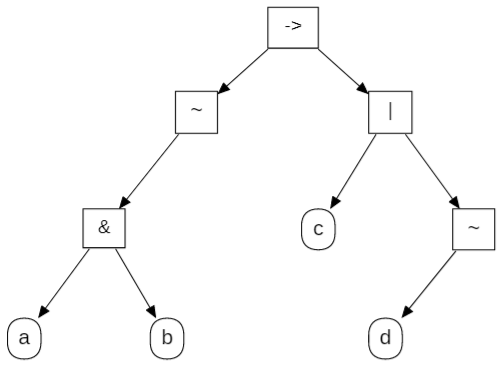
\includegraphics[width=0.7\textwidth, height=0.4\textheight]{img/albero.png}
\end{figure}
In questo albero, la radice è il nodo ``$->$'', perché è il connettivo principale della formula dell'esempio. I nodi ``$\thicksim$'' hanno solo il figlio sinistro perché rappresentano la negazione, e le foglie sono le atomiche \emph{a, b, c, d}.

La classe \texttt{CompoundFormula} ha quindi come attributi il campo \texttt{mainConnective} che definisce il connettivo principale, e il campo \texttt{subFormulas} che consiste in un array di formule che contiene i nodi figli. La classe contiene dei metodi getter per ottenere il connettivo, il figlio destro ed il figlio sinistro, e sovrascrive i metodi \texttt{toString} e \texttt{toCnf}.

\section{Clausificazione di una formula}
\label{clausification}
Come spiegato all'inizio di questo capitolo, se volessimo verificare la soddisfacibilità di una formula \emph{F} tramite il metodo di risoluzione, è fondamentale effettuare prima la \emph{clausificazione} di \emph{F}, ovvero la sua conversione in \emph{CNF}, in modo tale da ottenere l'insieme di clausole necessario per il metodo di risoluzione. Per fare ciò bisogna applicare alcune regole di inferenza:
\begin{itemize}
    \item \textbf{Eliminazione della doppia implicazione}: 
    \[
    (p \tto q) \quad \equiv \quad ((p \to q) \land (q \to p))
    \]
    
    \item \textbf{Eliminazione dell'implicazione}: 
    \[
    (p \to q) \quad \equiv \quad (\lnot p \lor q)
    \]
    
    \item \textbf{Proprietà distributiva di or su and}:
    \[
    (p \lor (q \land r)) \quad \equiv \quad ((p \lor q) \land (p \lor r))
    \]
    
    \item \textbf{Doppia negazione}:
    \[
    \lnot\lnot p \quad \equiv \quad p
    \]
    
    \item \textbf{Leggi di De Morgan}:
    \[
    \lnot(p \land q) \quad \equiv \quad (\lnot p \lor \lnot q)
    \]
    \[
    \lnot(p \lor q) \quad \equiv \quad (\lnot p \land \lnot q)
    \]
\end{itemize}
Le regole appena mostrate vengono applicate nel metodo astratto \texttt{toCnf} della classe \texttt{Formula}, che restituisce un \texttt{ClauseSet}. Questo metodo ha quindi due diverse implementazioni: una per le formule atomiche e una per le formule composte.

L'implementazione del metodo \texttt{toCnf} nella classe \texttt{AtomicFormula} è molto semplice: esso restituisce un \texttt{ClauseSet} contenente una sola clausola, tale clausola contiene soltanto il letterale associato a quella formula atomica.
 
L'implementazione del metodo nella classe \texttt{CompoundFormula} invece applica sulla formula le regole di inferenza sopra citate, seguendo un approccio ricorsivo. Per la creazione del \texttt{ClauseSet} da restituire, utilizza i metodi \texttt{union} delle classi \texttt{Clause} e \texttt{ClauseSet}.

\subsection{Esempio di clausificazione}
Consideriamo la seguente formula:
\[ (a \lor b) \to c \]
la clausificazione viene fatta in tre passaggi:

\begin{itemize}
    \item Eliminazione implicazione:
    \[ \lnot (a \lor b) \lor c \]
    \item De Morgan:
    \[ (\lnot a \land \lnot b) \lor c \]
    \item Proprietà distributiva:
    \[ (\lnot a \lor c) \land (\lnot b \lor c) \]
\end{itemize}

La formula ricavata nell'ultimo passaggio è in \emph{CNF}, ed essa corrisponde all'insieme di clausole:
\[ \{ \; \{\lnot a, c\}; \{\lnot b, c\} \; \} \]

\section{Parsing di formule}
\label{parsing}
Se volessimo utilizzare un programma che legge da un flusso di input una formula in formato testuale (ad esempio da \emph{Stdin} o da un file di testo), è necessario interpretare la stringa di testo in modo tale da ottenere la formula. La trasformazione di rappresentazioni testuali in strutture dati utilizzabili da un programma è un processo noto come \emph{parsing}. Nel nostro sistema, implementiamo un parser per convertire le formule da stringhe di testo in oggetti di tipo \texttt{Formula}. Per eseguire il parsing, bisogna definire prima una grammatica che descrive il linguaggio utilizzato per le formule. A partire dalla grammatica vengono generati il \emph{lexer}, il \emph{parser} e il \emph{listener}.


\subsection{Utilizzo del parser ANTLR4}
Il parser utilizzato nel nostro sistema è \emph{ANTLR4}. Nella struttura del progetto presente nella sezione \ref{project_structure}, nel package \emph{antlr4} è presente il file \emph{FormulaExpression.g4} che contiene la grammatica. Inoltre, sono presenti quattro file che sono stati generati automaticamente da \emph{ANTLR4} a partire dalla grammatica:
\begin{itemize}
    \item \textbf{FormulaExpressionLexer.java}:
    esso consiste nel lexer, ovvero l'analizzatore lessicale; il suo scopo è quello di analizzare la stringa in input ed ottenere da esso un flusso di \emph{token}. In questo caso i token sono i connettivi, le variabili atomiche, e i caratteri di \emph{white space}.
    \item \textbf{FormulaExpressionParser.java}:
    esso consiste nel parser, che esegue l'analisi sintattica della stringa in input generando un \textbf{albero sintattico} (\emph{AST}), fondamentale per la costruzione della formula.
    \item \textbf{FormulaExpressionListener.java}:
    è un interfaccia che definisce i metodi che vengono richiamati durante l'attraversamento dell'\emph{AST}.
    \item \textbf{FormulaExpressionBaseListener.java}:
    è una classe che implementa l'interfaccia \texttt{FormulaExpressionListener}, dove ogni metodo sovrascritto non esegue alcuna operazione.
\end{itemize}

Oltre a questi file, ne sono presenti altri due:
\begin{itemize}
    \item \textbf{FormulaListenerImplementation.java}:
    è una classe che estende il Base Listener. Utilizza uno \emph{stack} di formule come campo per la creazione delle sottoformule, e sovrascrive alcuni metodi del Base Listener.
    \item \textbf{ParseFormula.java}:
    è una classe che contiene soltanto il metodo \texttt{parse}. Esso è il metodo principale che prende in input una stringa, e mette insieme tutte le componenti viste precedentemente, creando tutto l'occorrente per il parsing. Infine restituisce la formula ottenuta a partire dalla stringa in input.
\end{itemize}

\subsubsection{La grammatica utilizzata}

Nel codice \ref{grammar} è presente il contenuto del file \emph{FormulaExpression.g4} che descrive la grammatica.

\begin{minipage}{\linewidth}
    \begin{lstlisting}[label=grammar, caption={file FormulaExpression.g4}]
        grammar FormulaExpression;

        start : formula EOF;

        formula : atomic_formula
                | '(' formula ')' 
                | unary_connective formula
                | formula binary_connective formula
                ;

        atomic_formula : LITERAL ;

        unary_connective : NOT ;

        binary_connective : AND | OR | IMPLIES | IFF;

        //token
        AND : '&' ;
        OR : '|' ;
        IMPLIES : '->' ;
        NOT : '~' ;
        IFF : '<->';

        LITERAL : [a-z]+ ;
        WS : [ \t\r\n]+ -> skip ;
    \end{lstlisting}
\end{minipage}
In questa grammatica ci sono le regole che definiscono le formule atomiche e composte, e le regole che descrivono i connettivi unari e binari; le sottoformule sono distinguibili grazie alle parentesi tonde, che specificano anche la precedenza tra i vari connettivi della formula. in fondo al file è presente la definizione dei token. È bene notare che la rappresentazione testuale dei connettivi in questa grammatica è la medesima utilizzata dall'enumerazione \texttt{Connective}.

\subsubsection{Esempio di \emph{AST}}
Consideriamo la seguente stringa:
\[ (a \; \& \; \sim b) \quad -> \quad c \]
se eseguiamo il parsing di questa stringa otteniamo il seguente \emph{AST}:
\begin{figure}[H]
    % \centering
    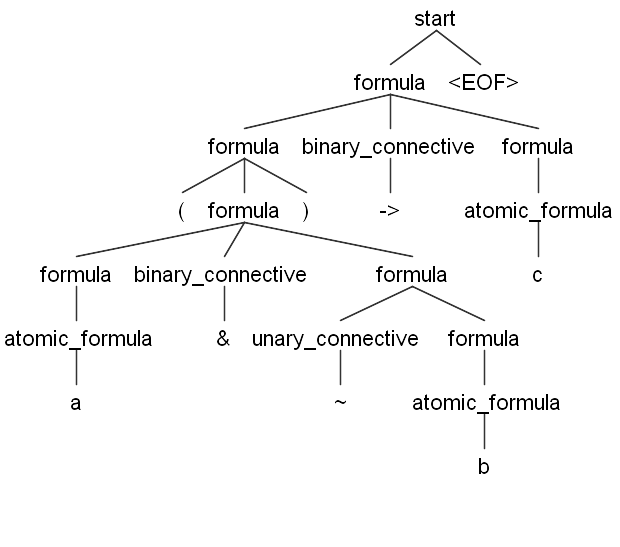
\includegraphics[width=0.7\textwidth, height=0.5\textheight]{img/antlr4_parse_tree.png}
\end{figure}
Durante l'attraversamento di questo albero vengono eseguiti i metodi \\ \texttt{ExitAtomic\_formula} e \texttt{exitFormula} della classe che estende il Base Listener; essi vengono richiamati rispettivamente quando si esce da un nodo \emph{atomic\_formula} e da un nodo \emph{formula}. Nel primo caso si crea una formula atomica e la si aggiunge allo \emph{stack} (tramite l'operazione di \emph{push}), nel secondo caso si controlla la presenza di un figlio che contiene un connettivo unario o binario, e si crea una formula composta applicando quel connettivo alla formula in cima allo stack (nel caso di connettivo unario) oppure alle prime due formule in cima allo stack (nel caso di connettivo binario). Infine viene inserita nello stack la formula appena creata. Per ottenere l'elemento in cima allo stack viene usata l'operazione di \emph{pop} su di esso.

Alla fine della visita dell'\emph{AST}, in cima allo stack ci sarà la formula associata alla stringa di partenza, che viene ottenuta dal metodo \texttt{getFormula} e a sua volta restituita dal metodo \texttt{parse} (si veda il codice \ref{parse}). Nell'esempio visto in precedenza la formula ottenuta è:
\[ (a \land \lnot b) \to c \]

\begin{minipage}{\linewidth}
    \begin{lstlisting}[caption={Metodo \texttt{parse} della classe \texttt{ParseFormula}}, label={parse}]
        public static Formula parse(String formulaStr) {
            CharStream input = CharStreams.fromString(formulaStr);
            FormulaExpressionLexer lexer = new FormulaExpressionLexer(input);
            CommonTokenStream tokens = new CommonTokenStream(lexer);
            FormulaExpressionParser parser = new FormulaExpressionParser(tokens);

            //create listener
            FormulaListenerImplementation listener = new FormulaListenerImplementation();

            //adds the listener to the parser
            parser.addParseListener(listener);

            try {
                //analyze the input and get the corresponding formula
                parser.start();
                return listener.getFormula();
            } catch (Exception e) {
                return null;
            }
        }
    \end{lstlisting}
\end{minipage}


% 
% 
%			CAPITOLO 5
\chapter{Logiche modali non-normali ed estensione del metodo di risoluzione}
\label{modal}
Questo capitolo si concentra sulle logiche modali e su come estendere il metodo di risoluzione per questo tipo di logiche. La prima parte del capitolo illustra le nozioni teoriche, la seconda parte riguarda l'implementazione in Java di quello che viene spiegato nella parte teorica. 

\section{Panoramica sulle logiche modali non-normali}
Le logiche modali \emph{non-normali} (\emph{NNML}) sono una classe di sistemi logici che estendono la logica modale normale introducendo concetti e assiomi che non sono presenti nella forma più basilare della logica modale. Queste logiche \emph{non-normali} si discostano dalle proprietà della logica modale \emph{normale} minima, \textbf{K}, che soddisfa tutti gli assiomi basilari della logica modale. Queste logiche sono organizzate gerarchicamente in un ``cubo'' di sistemi logici, che comprende la logica modale \textbf{E} come la più semplice e altre logiche ottenute aggiungendo assiomi come \textbf{C}, \textbf{M} e \textbf{N}. Il metodo di risoluzione che vediamo in questo capitolo si concentra soltanto sulla logica modale non-normale minimale \textbf{E}.

Le formule delle logiche modali (normali e non-normali) utilizzano, oltre ai connettivi della logica classica, il connettivo \emph{box} ($\Box$); Questo connettivo è fondamentale nella formalizzazione di concetti come la necessità, l'obbligatorietà, la conoscenza o la verità assoluta, a seconda del contesto in cui viene utilizzato.

\section{Forma clausale}
La forma clausale di una formula consiste in un insieme di clausole, come nel caso della logica classica.
\subsection{Letterali}
I letterali possono essere di due tipi: \emph{proposizionali} o \emph{modali}. I letterali proposizionali sono i medesimi della logica classica (si veda sezione \ref{CNF}); i letterali modali sono della forma $\Box p$ oppure $\lnot \Box p$, dove $p$ è una variabile proposizionale.
\subsection{Clausole}
Le clausole, come nella logica classica, sono una disgiunzione di letterali. Questa volta però le clausole possono essere di due tipi: 
\begin{itemize}
    \item \textbf{Clausola locale}: \[ l_1 \lor l_2 \lor \ldots \lor l_n \]
    \item \textbf{Clausola globale}: \[ G(l_1 \lor l_2 \lor \ldots \lor l_n) \]
\end{itemize}
dove $l_i$ è un letterale proposizionale o modale. Una clausola globale è vera in tutti i mondi di un modello, una clausola locale invece è vera soltanto in un mondo del modello.

\section{Clausificazione di formule modali}
Per poter effettuare la clausificazione di una formula $\phi$ è necessario utilizzare una funzione $\eta$ il cui scopo è quello di associare una nuova variabile proposizionale ad ogni sottoformula di $\phi$. La funzione $\eta$ si utilizza all'interno di un'altra funzione, chiamata \textbf{R}, che è la funzione di riduzione. La clausificazione della formula $\phi$ viene fatta in questo modo:
\[ \{ \eta(\phi) \} \cup R(G(\eta(\phi) \tto \phi)) \]
dove \textbf{R} è definita in questo modo:
\[
\begin{aligned}
R(G(t \tto p)) &= \{ G(\lnot t \lor p), G(t \lor \lnot p) \} \\
R(G(t \tto \lnot \psi)) &= \{ G(\lnot t \lor \lnot \eta(\psi)), G(t \lor \eta(\psi)) \} \cup R(G(\eta(\psi) \tto \psi)) \\
R(G(t \tto \psi \lor \psi')) &= \{ G(\lnot t \lor \eta(\psi) \lor \eta(\psi')), G(t \lor \lnot \eta(\psi)), G(t \lor \lnot \eta(\psi')) \} \\
& \quad \cup R(G(\eta(\psi) \tto \psi)) \cup R(G(\eta(\psi') \tto \psi')) \\
R(G(t \tto \Box \psi)) &= \{ G(\lnot t \lor \Box \eta(\psi)), G(t \lor \lnot \Box \eta(\psi)) \} \cup R(G(\eta(\psi) \tto \psi))
\end{aligned}
\]
La clausola {$\eta(\phi)$} è una clausola locale che contiene soltanto la variabile proposizionale associata alla formula $\phi$.      L'insieme di clausole che contiene solo questa clausola viene unito all'insieme di clausole ottenuto ricorsivamente dalla funzione \emph{R} applicata alla formula globale $G(\eta(\phi) \tto \phi)$. Si noti che questa funzione è definita solamente per i connettivi \emph{not}, \emph{or} e \emph{box}. Gli altri connettivi binari possono essere trasformati in \emph{or}.

\subsection{Esempio di clausificazione}

\section{Metodo di Risoluzione per logiche modali}
\subsection{Regole di inferenza per la logica modale \emph{E}}

\section{Implementazione della forma clausale}

\section{implementazione delle formule modali}
\subsection{Implementazione della clausificazione}

\section{Implementazione del metodo di risoluzione}

















% 
% 
%			CAPITOLO 6
\chapter{Applicazioni pratiche del metodo di risoluzione}
\label{app}

\section{Verificare la validità di una formula}
\section{Dimostrazione di conseguenze logiche}
\section{Dimostrazione di equivalenze logiche}

% 
% 
%			CAPITOLO 7
\chapter{Testing}
\label{testing}

\section{Struttura del file di test}

% 
% 
%			CAPITOLO 8
\chapter{Conclusioni}
\label{conclusion}

%
%			BIBLIOGRAFIA
%
\begin{thebibliography}{00}

% esempio di bibliografia:


%
\bibitem{esempio}
...
%
% \bibitem{gotti91}
% M. Gotti, I linguaggi specialistici, Firenze, La Nuova Italia, 1991.
% %
% \bibitem{wellek62}
% R. Wellek, A. Warren, Theory of Literature , 3rd edition, New York, Harcourt, 1962.
% %
% \bibitem{canziani78}
% A. Canziani et al., Come comunica il teatro: dal testo alla scena. Milano, Il Formichiere, 1978.
% %
% \bibitem{MoD67}
% Ministry of Defence, Great Britain, Author and Subject Catalogues of the Naval Library, London, Ministry of Defence, HMSO, 1967.
% %
% \bibitem{heine23}
% H. Heine, Pensieri e ghiribizzi. A cura di A. Meozzi. Lanciano, Carabba, 1923.
% %
% \bibitem{basso62}
% L. Basso, ``Capitalismo monopolistico e strategia operaia'', Problemi del socialismo, vol. 8, n. 5, pp. 585-612, 1962.
% %
% \bibitem{avirovic93}
% L. Avirovic, J. Dodds (a cura di), Atti del Convegno internazionale ``Umberto Eco, Claudio Magris. Autori e traduttori a confronto'' ( Trieste, 27-28 novembre 1989), Udine, Campanotto, 1993.
% %
% \bibitem{gans67}
% E.L. Gans, "The Discovery of Illusion: Flaubert's Early Works, 1835-1837", unpublished Ph.D. Dissertation, Johns Hopkins University, 1967.
% %
% \bibitem{harrison92}
% R. Harrison, Bibliography of planned languages (excluding Esperanto).  \url{http://www.vor.nu/langlab/bibliog.html}, 1992, agg. 1997.
%
\end{thebibliography}
% 

%
%			RINGRAZIAMENTI
%
\prefacesection{Ringraziamenti}
...

\end{document}


 
